\chapter{Lecture-1 May, 18, 2021}
\textbf{Soft computing} is also known as Artificial Intelligent, AI, which is a new concept comparing to the conventional model-based \textbf{hard computing}.
There are 3 types of soft computing models:
\begin{enumerate}
\item \textbf{Neural Networks} \& Machine learning
\begin{itemize}
\item Data Driven, Learn from data
\item \textbf{Limit}: not good on non-numerical data
\end{itemize}
\item \textbf{Fuzzy Systems}, which mimics human decision 
\begin{itemize}
\item Use experience or expert knowledge through Fuzzy rules
\item \textbf{Limit}: difficult to handle the uncertainties not in the knowledge domain
\end{itemize}
\item \textbf{Genetic Algorithm} (GA), Simulated Annealing (SA), Particle Swarm Optimization (PSO), \colorbox{Orange}{ACO(???)} and Artificial Immune System (AIS).
\begin{itemize}
\item Use evolutionary computing method to provide the optimal solutions
\item \textbf{Limit}: normally very slow
\end{itemize}
\end{enumerate}
\\
\textcolor{red} {These 3 types of mythologies are complementary, based on your specific application or problem, choose the MOST suitable method, or combining some of them, including traditional methods. The proposed solution should be better or least on some aspects better than existing solutions} 

\noindent{\color{red} \rule{\linewidth}{0.5mm}}
% ====================================================================================
\section{Neural Networks}

There are two types of Neural Networks (NN):
\begin{itemize}
    \item Biological NN: based on biological structure
    \item Artificial NN: less biological structure, more like a math unit
\end{itemize}

There are three types of learning for neural networks:
\begin{enumerate}
    \item Supervised Learning: where the supervisor is always available to tell the \textcolor{red}{error} and the learning is to reduce errors
    \item Unsupervised Learning: no supervisor, learning is based on the feature of objects. E.g. classifying apples into Good, Normal, Bad categorise. This type of learning is mainly used for classification/recognition. There is \textcolor{red}{no error} involved here
    \item Reinforcement Learning: No errors/feedback at all the time, however, it has a \textcolor{red}{delayed and overall score/feedback}.
\end{enumerate}
\noindent{\color{red} \rule{\linewidth}{0.5mm}}


% ====================================================================================
\section{The Model of A Single Neuron}
For a neuron, it has many inputs, but only one output. \(x_1\), \(x_2\), ... \(x_N\) are the input from other N neurons. \(w_1\),\(w_2\), ... ,\(w_N\),  are the connection weights.

\begin{equation}
  \textrm{Total Input} = \sum_{i=1}^{N} w_i x_i   
\end{equation}

\begin{center}
\begin{tikzpicture}
\Vertex[x=1,label=\(x_1\)]{A} 
\Vertex[x=2,label=\(x_2\)]{B}
\Vertex[x=3,label=\(x_3\)]{C}
\Vertex[x=4,label=...]{D} 
\Vertex[x=5,label=\(x_N\)]{DD} 
\Vertex[x=3,y=-2,label=Neuron,size = 1]{E}
\Vertex[x=3,y=-4, label=y]{F}

\Edge[bend=-10,Direct=true,label=w1](A)(E)
\Edge[bend=-5,Direct=true,label=w2](B)(E)
\Edge[bend=5,Direct=true,label=w3](C)(E)
\Edge[bend=10,Direct=true,label=...](D)(E)
\Edge[bend=10,Direct=true,label=\(w_N\)](DD)(E)
\Edge[bend=0,Direct=true](E)(F)
\end{tikzpicture}
\end{center}
One fundamental important thing for a neuron is it has a threshold, let $\theta$ be the threshold, $f(...)$ is the activation function, also called input-output function, we have the one neuron model as:
\begin{equation}
 y = f(\sum_{i=1}^{N} w_i x_i - \theta)  
\end{equation}
\noindent{\color{red} \rule{\linewidth}{0.5mm}}
% ====================================================================================
\section{Commonly used activation functions}

There are 6 types of commonly used activation functions:
\subsection{Linear}: \[y = f(x) = x\]
\begin{center}
\begin{tikzpicture}
  \draw[->] (-3, 0) -- (3, 0) node[right] {$x$};
  \draw[->] (0, -3) -- (0, 3) node[above] {$y$};
  \draw[scale=0.8, domain=-3:3, smooth, variable=\x, blue] plot ({\x}, {\x});
%   \draw[scale=0.5, domain=-3:3, smooth, variable=\y, red]  plot ({\y*\y}, {\y});
\end{tikzpicture}
\end{center}

\subsection{Hard Limiter, HL}
\[y = f(x) = \left\{ {\begin{array}{*{20}{c}}
{1{\textrm{ if }}x \ge 0}\\
{ - 1{\textrm{ if }}x < 0}
\end{array}} \right. = {\rm{sign}}(x)\]

\begin{center}
\begin{tikzpicture}
  \draw[->] (-3, 0) -- (3, 0) node[right] {$x$};
  \draw[->] (0, -3) -- (0, 3) node[above] {$y$};
  \draw[scale=1, domain=-3:0, smooth, variable=\x, blue] plot ({\x}, {-1});
  \draw[scale=1, domain=0:3, smooth, variable=\x, blue] plot ({\x}, {1});
\end{tikzpicture}
\end{center}

Alternatively, this can be written as:

\[y = f(x) = \left\{ {\begin{array}{*{20}{c}}
{1{\textrm{ if }}x \ge 0}\\
{ 0 {\textrm{ if }}x < 0}
\end{array}} \right.\]

\subsection{Ramplimitter, piecewise limitter}
\[y = f(x) = \left\{ {\begin{array}{*{20}{c}}
F&{if}&{x \ge F}\\
x&{if}&{ - F \le x \le F}\\
{ - F}&{if}&{x \le F}
\end{array}} \right.\]
\begin{center}
\begin{tikzpicture}
  \draw[->] (-3, 0) -- (3, 0) node[right] {$x$};
  \draw[->] (0, -3) -- (0, 3) node[above] {$y$};
  \draw[scale=1, domain=-3:-1, smooth, variable=\x, blue] plot ({\x}, {-1});
  \draw[scale=1, domain=-1:1, smooth, variable=\x, blue] plot ({\x}, {\x});
  \draw[scale=1, domain=1:3, smooth, variable=\x, blue] plot ({\x}, {1});
  \filldraw[black] (1,1) circle (2pt) node[anchor=south] {(F,F)};
   \filldraw[black] (-1,-1) circle (2pt) node[anchor=north] {(-F,-F)};
\end{tikzpicture}
\end{center}

\subsection{Sigmoid, the most popular and commonly used function}
\[{y_1} = \frac{{{e^x} - {e^{ - x}}}}{{{e^x} + {e^{ - x}}}} = \tanh (x)\]
\[{y_2} = \frac{1}{{1 + {e^{ - x}}}}\]
\[\begin{array}{l}
{y_2} = \frac{1}{2}\left( {{y_1} + 1} \right)\\
{y_1} = 2\left( {{y_2} - 0.5} \right)
\end{array}\]
\begin{center}
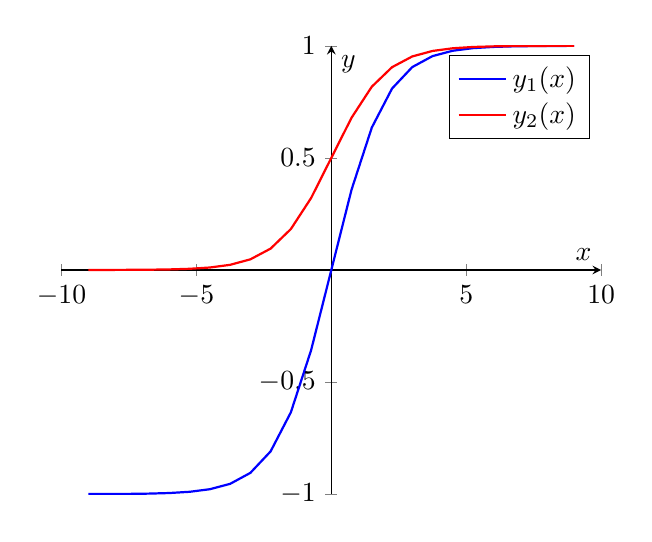
\begin{tikzpicture}[declare function={sigma2(\x)=1/(1+exp(-\x));
sigma1(\x)=2*sigma2(\x)-1;}]
\begin{axis}%
[
    % grid=major,     
    xmin=-10,
    xmax=10,
    axis x line=middle,
    ytick={-1,-0.5,0,0.5,1},
    ymax=1,
    ymin = -1,
    axis y line=middle,
    xlabel={$x$},
    ylabel={$y$}]
    samples=1000,
    
    legend style={at={(1,0.9)}}     
]
    \addplot[domain=-9:9,blue,mark=none,thick]   (x,{sigma1(x)});
    \addplot[domain=-9:9,red,mark=none,thick]   (x,{sigma2(x)});
    \legend{$y_1(x)$,$y_2(x)$}
\end{axis}
\end{tikzpicture}
\end{center}
\subsection{Linear-Above Threshold}
\[y = f\left( x \right) = {\left[ x \right]^ + } = \left\{ {\begin{array}{*{20}{c}}
x&{if}&{x \ge 0}\\
{}&{}&{}\\
0&{if}&{x < 0}
\end{array} = \max \left( {0,x} \right)} \right.\]
\begin{center}
    \begin{tikzpicture}
\begin{axis}[
    axis lines=middle,
    xmax=6,
    xmin=-6,
    ymin=-0.05,
    ymax=5.05,
    xlabel={$x$},
    ylabel={$y$}]
\addplot [domain=-5.5:5.5, samples=100, thick, blue] {max(0, x)};
\end{axis}
\end{tikzpicture}
\end{center}
\subsection{Linear-Below Threshold}

\[y = f\left( x \right) = {\left[ x \right]^ - } = \left\{ {\begin{array}{*{20}{c}}
0&{if}&{x \ge 0}\\
{}&{}&{}\\
{ - x}&{if}&{x < 0}
\end{array} = \max \left( {0, - x} \right)} \right.\]
\begin{center}
    \begin{tikzpicture}
\begin{axis}[
    axis lines=middle,
    xmax=6,
    xmin=-6,
    ymin=-0.05,
    ymax=5.05,
    xlabel={$x$},
    ylabel={$y$}]
\addplot [domain=-5.5:5.5, samples=100, thick, blue] {max(0, -x)};
\end{axis}
\end{tikzpicture}
\end{center}
\noindent{\color{red} \rule{\linewidth}{0.5mm}}
% ====================================================================================
\section{Model of A Single Layer Neural Network}
For a \textcolor{red}{fully connected} single layer neural network has M neurons (M outputs) and N inputs,
for the 1st neuron, we have:
\[{y_1} = f(\sum\limits_{i = 1}^N {{w_{1i}}} {x_i} - {\theta _1})\]
for the jth neuron, we have:
\[{y_j} = f(\sum\limits_{i = 1}^N {{w_{ji}}} {x_i} - {\theta _j})\]
where j could be any number between 1 to M.
\\
\\
If we choose $ - {\theta _j} = {x_0} {w_{j0}}$:  i.e. $x_0 \equiv 1$, and then, $w_{j0}\equiv-\theta_0$
Then, the argument-ed y becomes:
\[{y_j} = f(\sum\limits_{i = 0}^N {{w_{ji}}} {x_i})\]
where j could be any number between 0 to M, j = 0 for is the threshold.
\begin{center}
\begin{tikzpicture}
\Vertex[x=0,size=1,RGB,color={190,174,212},label=$x_0\equiv1$]{AA} 
\Vertex[x=2,size=1,label=$x_1$]{A} 
\Vertex[x=4,size=1,label=\(x_2\)]{B}
\Vertex[x=6,size=1,label=\(...\)]{C}
\Vertex[x=8,size=1,label=\(x_i\)]{D} 
\Vertex[x=10,size=1,label=\(...\)]{E}
\Vertex[x=12,size=1,label=\(x_N\)]{F}



\Vertex[x=4,y=-3,label=1,size = 1]{G}
\Vertex[x=4,y=-5, label=y1]{H}

\Vertex[x=7.5,y=-3,label=...,size = 1]{I}
\Vertex[x=7.5,y=-5, label=\(y_j\)]{J}

\Vertex[x=10,y=-3,label=M,size = 1]{K}
\Vertex[x=10,y=-5, label=\(y_M\)]{L}

\Edge[bend=-10,Direct=true,label=w10](AA)(G)
\Edge[bend=-10,Direct=true,label=w11](A)(G)
\Edge[bend=-5,Direct=true,label=w12](B)(G)
\Edge[bend=5,style={dashed},Direct=true,label=...](C)(G)
\Edge[bend=10,Direct=true,label=\(w_{1i}\)](D)(G)
\Edge[bend=10,style={dashed},Direct=true,label=\(...\)](E)(G)
\Edge[bend=10,Direct=true,label=\(w_{1N}\)](F)(G)

\Edge[bend=80,Direct=true,color=red,label=\(w_{ji}\)](D)(I)
\Edge[bend=-60,Direct=true,color=red,label=$w_{j0}\equiv-\theta_j$](AA)(I)
\Edge[bend=0,Direct=true](G)(H)
\Edge[bend=0,Direct=true](I)(J)
\Edge[bend=0,Direct=true](K)(L)
\end{tikzpicture}
\end{center}
\\
Write in the compact format: $\mathbb{Y}=f(\mathbb{W}\mathbb{X}^*)$, where $\mathbb{X}^*$ is a N+1 by 1 vector. $\mathbb{W}$ is the weight matrix with size M by N+1

\[\mathbb{W} = \left( {\begin{array}{*{20}{c}}
{{w_{10}}}&{{w_{11}}}& \cdots &{{w_{1N}}}\\
{{w_{20}}}&{w_{21}}}& \cdots &{{w_{2N}}}\\
 \vdots & \vdots & \ddots & \vdots \\
{{w_{M0}}}&{{w_{M1}}}& \cdots &{{w_{MN}}}
\end{array}} \right)\]

\noindent{\color{red} \rule{\linewidth}{0.5mm}}
% ====================================================================================
\section{Multi-Layer Neural Network Structure}
3-layer neural network is the most popular choice, actually there are only 2 layer of neurons (input layers which are not neurons, plus one layer of hidden neurons, and one layer of output neurons)
For a fully connected 3 layers neural network has M outputs, Q hidden neurons, and N inputs:
\[
\mathbb{H}=g(\mathbb{V}\mathbb{X}^*)
\]
\[
\mathbb{Y}=f(\mathbb{W}\mathbb{H}^*)
\]
\noindent{\color{red} \rule{\linewidth}{0.5mm}}
\\
5-layer neural network has one input layer, 3 hidden layer and 1 output layer:
\[
\mathbb{H_1}=g(\mathbb{V}\mathbb{X}^*)
\]
\[
\mathbb{H_2}=g(\mathbb{V_1}\mathbb{H_1}^*)
\]
\[
\mathbb{H_3}=g(\mathbb{V_2}\mathbb{H_2}^*)
\]
\[
\mathbb{Y}=f(\mathbb{W}\mathbb{H_3}^*)
\]
\noindent{\color{red} \rule{\linewidth}{0.5mm}}
% ====================================================================================
\section{Conclusion}
\begin{enumerate}
    \item the output activation function can be linear or non-linear
    \item the activation function for neurons in the hidden layer must be nonlinear
    \item the connections are only from layer i to i+1
    \item the thresholds are essentially important
\end{enumerate}